%%%%%%%%%%%%%%%%%%%%%%%%%%%%%%%%%%%%%%%%%
% Proceedings of the National Academy of Sciences (PNAS)
% LaTeX Template
% Version 1.0 (19/5/13)
%
% This template has been downloaded from:
% http://www.LaTeXTemplates.com
%
% Original author:
% The PNAStwo class was created and is owned by PNAS:
% http://www.pnas.org/site/authors/LaTex.xhtml
% This template has been modified from the blank PNAS template to include
% examples of how to insert content and drastically change commenting. The
% structural integrity is maintained as in the original blank template.
%
% Original header:
%% PNAStmpl.tex
%% Template file to use for PNAS articles prepared in LaTeX
%% Version: Apr 14, 2008
%
%%%%%%%%%%%%%%%%%%%%%%%%%%%%%%%%%%%%%%%%%

%----------------------------------------------------------------------------------------
%	PACKAGES AND OTHER DOCUMENT CONFIGURATIONS
%----------------------------------------------------------------------------------------

%------------------------------------------------
% BASIC CLASS FILE
%------------------------------------------------

%% PNAStwo for two column articles is called by default.
%% Uncomment PNASone for single column articles. One column class
%% and style files are available upon request from pnas@nas.edu.

%\documentclass{pnasone}
\documentclass{pnastwo}

%------------------------------------------------
% POSITION OF TEXT
%------------------------------------------------

%% Changing position of text on physical page:
%% Since not all printers position
%% the printed page in the same place on the physical page,
%% you can change the position yourself here, if you need to:

% \advance\voffset -.5in % Minus dimension will raise the printed page on the 
                         %  physical page; positive dimension will lower it.

%% You may set the dimension to the size that you need.

%------------------------------------------------
% GRAPHICS STYLE FILE
%------------------------------------------------

%% Requires graphics style file (graphicx.sty), used for inserting
%% .eps/image files into LaTeX articles.
%% Note that inclusion of .eps files is for your reference only;
%% when submitting to PNAS please submit figures separately.

%% Type into the square brackets the name of the driver program 
%% that you are using. If you don't know, try dvips, which is the
%% most common PC driver, or textures for the Mac. These are the options:

% [dvips], [xdvi], [dvipdf], [dvipdfm], [dvipdfmx], [pdftex], [dvipsone],
% [dviwindo], [emtex], [dviwin], [pctexps], [pctexwin], [pctexhp], [pctex32],
% [truetex], [tcidvi], [vtex], [oztex], [textures], [xetex]

\usepackage{graphicx}

%------------------------------------------------
% OPTIONAL POSTSCRIPT FONT FILES
%------------------------------------------------

%% PostScript font files: You may need to edit the PNASoneF.sty
%% or PNAStwoF.sty file to make the font names match those on your system. 
%% Alternatively, you can leave the font style file commands commented out
%% and typeset your article using the default Computer Modern 
%% fonts (recommended). If accepted, your article will be typeset
%% at PNAS using PostScript fonts.

% Choose PNASoneF for one column; PNAStwoF for two column:
%\usepackage{PNASoneF}
%\usepackage{PNAStwoF}

%------------------------------------------------
% ADDITIONAL OPTIONAL STYLE FILES
%------------------------------------------------

%% The AMS math files are commonly used to gain access to useful features
%% like extended math fonts and math commands.


\usepackage{amssymb,amsfonts,amsmath}
\usepackage{chemfig,siunitx}
\setcompoundsep{7em}


%------------------------------------------------
% OPTIONAL MACRO FILES
%------------------------------------------------

%% Insert self-defined macros here.
%% \newcommand definitions are recommended; \def definitions are supported

%\newcommand{\mfrac}[2]{\frac{\displaystyle #1}{\displaystyle #2}}
%\def\s{\sigma}

%------------------------------------------------
% DO NOT EDIT THIS SECTION
%------------------------------------------------

% For PNAS Only:
\contributor{}
\url{https://www.dropbox.com/sh/zmlcek9to0yqfn5/NNJN9-vXDG}
\copyrightyear{2013}
\issuedate{Dec 12th}
\volume{0}
\issuenumber{0}

%----------------------------------------------------------------------------------------

\begin{document}

%----------------------------------------------------------------------------------------
%	TITLE AND AUTHORS
%----------------------------------------------------------------------------------------

\title{Characterization and Application of trans-cleaving hammerhead ribozymes} % For titles, only capitalize the first letter

%------------------------------------------------face
%% Enter authors via the \author command.  
%% Use \affil to define affiliations.
%% (Leave no spaces between author name and \affil command)

%% Note that the \thanks{} command has been disabled in favor of
%% a generic, reserved space for PNAS publication footnotes.

%% \author{<author name>
%% \affil{<number>}{<Institution>}} One number for each institution.
%% The same number should be used for authors that
%% are affiliated with the same institution, after the first time
%% only the number is needed, ie, \affil{number}{text}, \affil{number}{}
%% Then, before last author ...
%% \and
%% \author{<author name>
%% \affil{<number>}{}}

%% For example, assuming Garcia and Sonnery are both affiliated with
%% Universidad de Murcia:
%% \author{Roberta Graff\affil{1}{University of Cambridge, Cambridge,
%% United Kingdom},
%% Javier de Ruiz Garcia\affil{2}{Universidad de Murcia, Bioquimica y Biologia
%% Molecular, Murcia, Spain}, \and Franklin Sonnery\affil{2}{}}

\author{Ryan Tsoi\affil{1}{University of California, Berkeley},
Zackery Field\affil{1}{University of California, Berkeley}
}

\contributor{Submitted to Adam Arkin and Ron Weiss for review}

%----------------------------------------------------------------------------------------

\maketitle % The \maketitle command is necessary to build the title page

\begin{article}

%----------------------------------------------------------------------------------------
%	ABSTRACT, KEYWORDS AND ABBREVIATIONS
%----------------------------------------------------------------------------------------

\begin{abstract}

Our current ability to engineer biological circuits is hindered by the inability 
to design and create systems without unintended crosstalk or side interactions 
from a limited set of inducer-promoter pairs. This creates poor scalability of 
complex designs that are restricted by the number of well-characterized DNA regulators, 
and limits the overall complexity that can be encoded into a genetic circuit. 
To address these problems, we propose the use of RNA based logic as the building block 
for genetic engineering and replace inducer-promoter pairings with riboregulators such as ribozymes. 
RNA should be superior to DNA with regards to the goal of synthetic biology to produce 
safe, reliable, predictable, composable, tunable, and orthogonal genetic circuits. 
Two well-characterized circuits, the toggle switch and the repressilator, were investigated, 
and RNA-based equivalents were constructed from trans-cleaving hammerhead ribozymes. 
The outputs of the riboregulated toggle and repressilator were compared to their DNA counterparts, 
and it was found that the ribozyme systems did not achieve the desired output due to 
the fast rates of transcription and degradation of mRNA. This work introduces the prospect of 
using trans-cleaving ribozymes as a replacement for promoter and repressor protein pairs, 
and presents challenges that must be confronted in the future if genetic regulation by riboregulatory elements is 
to replace genetic regulation by protein regulatory elements.

\end{abstract}

%------------------------------------------------

\keywords{Synthetic Biology | Orthogonal part sets | Rational Logic Gate Design} % When adding keywords, separate each term with a straight line: |

%------------------------------------------------

%% Optional for entering abbreviations, separate the abbreviation from
%% its definition with a comma, separate each pair with a semicolon:
%% for example:
%% \abbreviations{SAM, self-assembled monolayer; OTS,
%% octadecyltrichlorosilane}

% \abbreviations{}
%\abbreviations{SAM, self-assembled monolayer; OTS, octadecyltrichlorosilane}

%----------------------------------------------------------------------------------------
%	PUBLICATION CONTENT
%----------------------------------------------------------------------------------------

%% The first letter of the article should be drop cap: \dropcap{} e.g.,
%\dropcap{I}n this article we study the evolution of ''almost-sharp'' fronts

\section{Introduction}

\dropcap{T}he world is currently facing a large variety of problems ranging from 
accessibility of environmentally friendly energy to curing disease, and researchers 
are looking to microorganisms as a possible solution due to the diversity in microbial 
species as well as genetic codes. It is believed that once these genetic codes 
are identified and understood, they can be manipulated to help solve these problems. ~\cite{promise}  

Over the past few decades, bacteria have been genetically engineered to produce a 
variety of compounds ranging from commodity chemicals to pharmaceuticals. 
They have been used in agriculture, medicine, bioremediation, and even treatments 
and therapies for complicated diseases like cancer. 

However, synthetic biology is still far from being an engineering science, and we 
can look to its macroscale analog electrical engineering to see why. Electrical 
engineers can use the same transistor or wire multiple times within the same 
circuit and achieve the desired output without undesired side interactions. ~\cite{microelectronics}
In contrast, current methods of genetic circuit design are limited by the 
inability to produce orthogonal systems from similar parts. 

Without physical barriers separating individual molecules or reactions, it is 
impossible to prevent crosstalk within the circuit and severely inhibits our 
ability to regulate these systems. As a result, effective circuit designs must 
contain all unique promoter-inducer combinations—this hinders the overall complexity 
that can be achieved but also is limited by the total number of identified 
and well-characterized pairings. 

We seek to address these concerns by proposing that researchers shift their focus 
within the central dogma of biology from protein-based regulators to RNA-based 
regulators for circuit design. While proteins are the most commonly investigated 
for synthetic biology applications, in many ways RNA is more suited to meet these 
design principles than proteins. 

For example, RNA is easier to design and tune because we can take advantage of 
Watson-Crick base pairing, whereas there has been minimal success in designing novel proteins. ~\cite{howfolds} ~\cite{protein_fold}
In addition, a wider variety of targets are available by simply knowing the 
DNA sequence of the target protein. Production and degradation of mRNA are 
faster than equivalent processes for protein, and mRNA production puts less 
energetic strain on the cell than protein production. ~\cite{protein_stress} ~\cite{RNA_stress}
Finally, physical properties such as open complex formation ~\cite{howfolds}, elongation, translation ~\cite{RBS_calc}, 
and degradation rates ~\cite{RNA_deg} can all be controlled in the mRNA itself. 

In this paper, we compare the advantages and disadvantages between riboregulators 
and protein regulators by looking at two equivalent versions of two different 
genetic circuits—a toggle switch ~\cite{DNA_toggle}, and a repressilator.
One uses hammerhead ribozymes regulating an mRNA circuit, and the other uses traditional 
promoter-repressor pairings. The repressilator is a synthetic genetic regulator network, 
which exhibits a stable oscillation similar to an electrical oscillator system with set time periods ~\cite{repressilator}. 
We model both circuits stochastically, and optimized tunable parameters to give the best output.  
Using both models, we test hypotheses concerning the ideal design principles mentioned 
previously and reach conclusions for the advantages of each type of circuit.

%------------------------------------------------

\section{Results}


\subsection{Implementation of RNA Toggle Switch Using trans-cleaving hammerhead ribozymes}


Two hammerhead ribozymes with corresponding cleavage sites on the opposing 
ribozymes were computationally designed for transcription in Escherichia coli 
and stochastically modeled in Java using the Gillespie algorithm in order to 
simulate an RNA logic toggle switch. The final system did not display switch-like 
behavior however, and the steady states of the ribozyme toggle switch were not
consistent with the classic toggle circuit. In the RNA circuit (See Fig. 1) , 
steady state concentrations of all species were consistently zero despite changing inlet parameters. 
At longer timescales, concentration of the species was dominated by degradation, 
as new ribozyme constructs produced by transcription participated immediately in 
binding and trans-cleaving of one another. As a result, the ribozyme in higher concentration 
would cleave all of the ribozyme in lower concentration, but inevitably degrade 
over the course of the reaction due to high RNA production and degradation rates 
relative to proteins. The system also lacked memory, a key characteristic of the 
toggle switch, which limited our designed circuit from being a true analog to the toggle circuit.


\subsection{Implementation of RNA Repressilator Using Ribozymes}

We also looked at incoporating three hammerhead ribozymes with corresponding cleavage 
sites into a circuit in a rock-paper-scissors fashion in order to closely simulate 
the repressilator by ~\cite{repressilator} in E. coli. This circuit was modeled 
stochastically in Matlab® using the Gillespie algorithm in order to observe how natural
variation would effect the stability of the system.

For the purposes of the model, the total amount of molecules and the time of 
reaction were kept low (biologically-unrealistic) in order to observe the 
oscillations of the RNA repressilator more clearly. In addition, the amplitude 
and the period of the oscillations were both tunable based on the rate of binding, 
rate of cleaving, and rate of production of our hammerhead ribozyme constructs. 

Comparing the RNA repressilator to the classic repressilator (see Figure 3.,4.), the 
time for one cycle of oscillations to complete for the ribozyme circuit (on the order of seconds) 
was significantly shorter than that of the DNA circuit (on the order of minutes). 
This difference in period of oscillations is not only a key difference but also explains 
why the oscillation’s minimum value in the ribozyme circuit is nonzero compared to the DNA repressilator. 
As the system varies between high concentrations of species A, B, and C, on average 
none of the ribozymes are not completely cleaved and removed from the system before 
the behavior of the system shifts to the next state. As a result, we see the oscillations 
shown in the figure where the number of molecules of each ribozyme varies between 
approximately 0.5 and 0.8 molecules on average.

While RNA is still a superior system than DNA in terms of its safety, 
composability, and tunability, our repressilator was extremely sensitive to 
noise caused by high degradation and production rates. The system failed to 
operate as desired, producing unstable, irregular oscillations at low concentrations 
of molecules. As a result, the circuit failed to meet most of the design 
criteria for biological circuit design, and additional parameters would need to 
be adjusted in order obtain an effective repressilator.

%------------------------------------------------

\section{Discussion}

As tertiary structure does for proteins, 2D and 3D structures of RNA molecules 
play a major role in the function of these molecules ~\cite{RNA_structure_function}.
There are many tools available the predict these higher order structures in 
RNA that are based on free-energy minimzation through WC base-pairing ~\cite{list_tools}.
The predictability of inter- and intra-RNA interactions plays a key role in the 
ability to tune the relative ribozyme activity (binding interactions), as well as 
the relative stability of a given ribozyme (introduce slow-acting cleaving sites). 
With all of these characteristics
of RNA in mind, we assumed that the use of a self-contained RNA regulator would 
be far better than the traditional use of promoter-repressor pairs in the modeling
of logic circuits biologically. This initial hypothesis was further supported
by the fact that RNA regulation would be on smaller timescales, which ramps up
the rate of signal transduction. 

One of the major challenges that we faced when modeling systems built with 
trans-cleaving hammerhead ribozymes is the lack of cooperativity
in these systems. There were many unknowns that came with designing and characterizing
a novel set of rationally designable parts. The hammerhead ribozymes themselves
are not new constructs, 

Instead, Michaelis–Menten kinetics best described
the relationship between the ribozyme and its substrate RNA (also a ribozyme in
our cases). 
The lack of cooperativity also resulted in the lack of
bistable modes in the modeled toggle switch. In the toggle switch the two
ribozymes cleaved each other $a_{RNA}$ $b_{RNA}$ As discussed above, any 

%----------------------------------------------------------------------------------------
%	MATERIALS AND METHODS
%----------------------------------------------------------------------------------------

%% Optional Materials and Methods Section
%% The Materials and Methods section header will be added automatically.

\begin{materials}

\subsection{Methods}

The modeling of the ribozyme toggle switch, and the ribozyme repressilator used
the same set of tools, and used the same process. The representative chemical reactions of each 
of these circuits designed by hand in a way that was equivalent to the original
toggle switch (Fig 2.) and repressilator design (Fig 3.). Each of these chemical
reactions given its own definition of likelihood based on its subtrate(s) and 
associated constants. These equations are then added to a Markov Chain simulator object.
When run, this object simulates random behavior by selecting two random numbers. The
first of which is used to portray the length of the next time step. After taking
into account the relaitve concentrations of each of the species and the resulting likelihood
of each of the reactions, the second random number is used to select the next reaction
to take place. So on each iteration the time in the model increases, and the chain
terminates upon the arrival at the endtime. 

Literature search revealed the likely rates at which each of the reactions was to 
occur. Necessary parameters that we had to determine included: transcription rates,
binding and diffusion rates of partially complimentary RNA strands, rate of
cleavage of hammerhead ribozymes, degradation of before and after cleavage.

Source is available here: https://github.com/zacatac/ribozyme-circuit-modeling


\subsection{Modeling Tools}

Java implementation of the Gillespie algorithm created by Anderson 
for his Genetic Devices course ~\cite{Anderson_Gillespie}.

Matlab implementation of the Gillespie algorithm created by Ryan Tsoi. 



\end{materials}

%----------------------------------------------------------------------------------------
%	APPENDICES (OPTIONAL)
%--------------------------------------------------------------------------------------Thanks to Jeremy and Sergey for their feedback....
%An appendix with a title.

%----------------------------------------------------------------------------------------
%	ACKNOWLEDGEMENTS
%----------------------------------------------------------------------------------------

\begin{acknowledgments}
Thanks to Jeremy and Sergey for their feedback.
\end{acknowledgments}

%----------------------------------------------------------------------------------------
%	BIBLIOGRAPHY
%----------------------------------------------------------------------------------------

%% PNAS does not support submission of supporting .tex files such as BibTeX.
%% Instead all references must be included in the article .tex document. 
%% If you currently use BibTeX, your bibliography is formed because the 
%% command \verb+\bibliography{}+ brings the <filename>.bbl file into your
%% .tex document. To conform to PNAS requirements, copy the reference listings
%% from your .bbl file and add them to the article .tex file, using the
%% bibliography environment described above.  

%%  Contact pnas@nas.edu if you need assistance with your
%%  bibliography.

%% Enter the largest bibliography number in the facing curly brackets
%% following \begin{thebibliography}


\begin{thebibliography}{10}
\bibitem{promise}
  Keasling J., {\em The Promise of Synthetic Biology}, The Bridge, 15 (2005),
  \url{http://www.nae.edu/Publications/Bridge/Cutting-EdgeResearchinEngineering/ThePromiseofSyntheticBiology.aspx}.

\bibitem{microelectronics}Madec, M.; Lallement, C.; Karstens, K.; Dittman, S.; Gersbacher, M.; Sorg, R.; Wild, M.; Muller, M.; Bourgine, P.; Donzeau, M.; Haiech, J., 
  {\em Synthetic biology and microelectronics: A similar design flow}, Circuits and Systems and TAISA Conference, 2009. NEWCAS-TAISA '09. Joint IEEE North-East Workshop on , vol., no., pp.1,4, June 28 2009-July 1 2009
  doi: 10.1109/NEWCAS.2009.5290444 

\bibitem{howfolds}Ignacio Tinoco Jr, Carlos Bustamante, How RNA folds, 
  Journal of Molecular Biology, Volume 293, Issue 2, 22 October 1999, 
  Pages 271-281, ISSN 0022-2836, http://dx.doi.org/10.1006/jmbi.1999.3001.

\bibitem{protein_fold}
  Onuchic, J.N. {\em et al.}, 
  {\em Theory of Protein Folding: The Energy Landscape perspective}, Annu. Rev. Phys. Chem. 1997.48:545-600, 
  \url{http://www.embnet.qb.fcen.uba.ar/embnet/references/frustra_ref1.pdf}

\bibitem{protein_stress}Diethard Mattanovich, Brigitte Gasser, Hubertus Hohenblum, Michael Sauer, 
  {\em Stress in recombinant protein producing yeasts}, Journal of Biotechnology, Volume 113, 
  Issues 1–3, 30 September 2004, Pages 121-135, ISSN 0168-1656, 
  \url{http://dx.doi.org/10.1016/j.jbiotec.2004.04.035}.

\bibitem{RNA_stress}Paulo P. Amaral, Marcel E. Dinger, and John S. Mattick
  {\em Non-coding RNAs in homeostasis, disease and stress responses: an evolutionary perspective}
  Briefings in Functional Genomics (2013) 12 (3): 254-278 doi:10.1093/bfgp/elt016

\bibitem{RBS_calc} Salis Lab, {\em RBS Calculator}, \url{http://salis.psu.edu/RBS_Calculator.shtml}

\bibitem{RNA_deg} Newbury S.F., {\em Control of mRNA stability in eukaryotes}, Biochemical Society Transactions (2006) 34, (30–34) (Printed in Great Britain) doi:10.1042/BST20060030

\bibitem{DNA_toggle} Gardner T.S. {\em et al.}, {\em Construction of a genetic toggle switch in E. coli}, Nature (2000) 403,
  \url{http://ender.bu.edu/~tgardner/be209/lectures/17/articles/gardner.ts_nature_1.20.00.pdf}

\bibitem{repressilator}Elowitz, Michael B.; Leibler, Stanislas, {\em A synthetic oscillatory network of transcriptional regulators}
  Nature 2000/01/20/print 403 335-338, \url{http://dx.doi.org/10.1038/35002125}

\bibitem{Anderson_Gillespie} Anderson J.C., {\em Java implementation of Gillespie}, Fall 2013 Devices Course

\bibitem{RNA_structure_function} Rebecca K. Montange and Robert T. Batey, 
  {\em Riboswitches: Emerging Themes in RNA Structure and Function}
  Annual Review of Biophysics, Vol. 37: 117 -133 (Volume publication date June 2008)

\bibitem{list_tools} \url{http://en.wikipedia.org/wiki/List_of_RNA_structure_prediction_software}


\end{thebibliography}

%----------------------------------------------------------------------------------------

\end{article}

%----------------------------------------------------------------------------------------
%	FIGURES AND TABLES
%----------------------------------------------------------------------------------------

%% Adding Figure and Table References
%% Be sure to add figures and tables after \end{article}
%% and before \end{document}

%% For figures, put the caption below the illustration.
%%
%% \begin{figure}
%% \caption{Almost Sharp Front}\label{afoto}
%% \end{figure}

%% For Tables, put caption above table
%%
%% Table caption should start with a capital letter, continue with lower case
%% and not have a period at the end
%% Using @{\vrule height ?? depth ?? width0pt} in the tabular preamble will
%% keep that much space between every line in the table.

%% \begin{table}
%% \caption{Repeat length of longer allele by age of onset class}
%% \begin{tabular}{@{\vrule height 10.5pt depth4pt  width0pt}lrcccc}
%% table text
%% \end{tabular}
%% \end{table}

%% For two column figures and tables, use the following:

%% \begin{figure*}
%% \caption{Almost Sharp Front}\label{afoto}
%% \end{figure*}

%% \begin{table*}
%% \caption{Repeat length of longer allele by age of onset class}
%% \begin{tabular}{ccc}
%% table text
%% \end{tabular}
%% \end{table*}

\begin{figure}    
  \label{fig1}
      \centering
       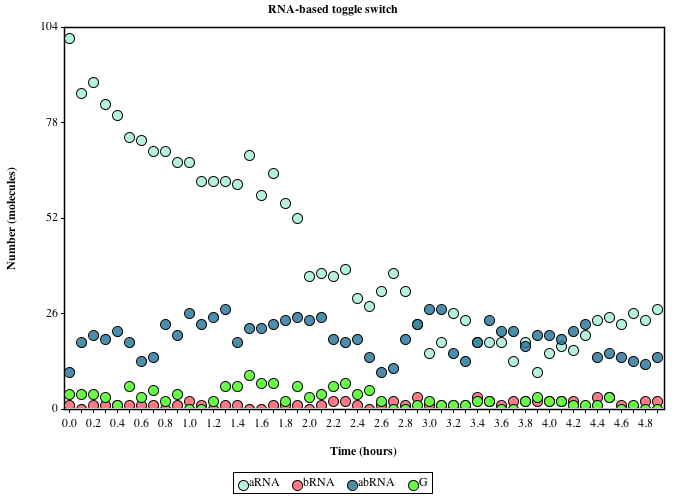
\includegraphics[width=0.4\textwidth]{RNA_based_toggle_timecourse.png}    
\caption{Example of timecourse showing the lack of stability given initial high concentration of $a_{\mbox{RNA}}$} 
\end{figure}

\begin{figure}
  \label{fig2}
  \centering
      \scalebox{0.7}{
      \schemestart
      $a_{DNA}$%\phantom{I}
      \arrow{->[$k_{a_{tc}}$]}
      $a_{RNA}$\phantom{}
      \arrow{<=>[*0$k_{a_{on}}$][*0$k_{a_{off}}$]}[-90]
      $a_{RNA}\cdot b_{RNA}$
      \arrow{<=>[*0$k_{b_{on}}$][*0$k_{b_{off}}$]}[-90]
      $b_{RNA}$
      \arrow{<-[$k_{b_{tc}}$]}[180]
      $b_{DNA}$
      \arrow(@c2--){->[$k_{a_{deg}}$]}
      $\emptyset$
      \arrow(@c3--){->[$k_{ab_{deg}}$]}
      $\emptyset$
      \arrow(@c4--){->[$k_{b_{deg}}$]}
      $\emptyset$
      \schemestop    
      }
\caption{Representative chemical process of the toggle switch. $a_{\mbox{RNA}}$
 and $b_{\mbox{RNA}}$ are both trans-cleaving hammerhead ribozymes. After
binding to one another, $a$ cleaves
$b$, and vice versa.}      
\end{figure}

\begin{figure}
\centering
      \scalebox{0.7}{
      \schemestart
      $a_{DNA}$%\phantom{I}
      \arrow{->[$k_{a_{tc}}$]}
      $a_{RNA}$\phantom{}
      \arrow{->[$k_{deg_a}$]}
      $\emptyset$
      \schemestop    
      }

      \scalebox{0.7}{
        \schemestart
        $b_{DNA}$%\phantom{I}
        \arrow{->[$k_{b_{tc}}$]}
        $b_{RNA}$\phantom{}
        \arrow{->[$k_{deg_b}$]}
        $\emptyset$
        \schemestop
      }

      \scalebox{0.7}{
        \schemestart
        $c_{DNA}$%\phantom{I}
        \arrow{->[$k_{c_{tc}}$]}
        $c_{RNA}$\phantom{}
        \arrow{->[$k_{deg_c}$]}
        $\emptyset$
        \schemestop
      }

      \scalebox{0.7}{
        \schemestart
        $a_{RNA}+b_{RNA}$%\phantom{I}
        \arrow{<=>[$k_{on_{ab}}$][$k_{off_{ab}}$]}
        $a_{RNA}\cdot b_{RNA}$\phantom{}
        \arrow{->[$k_{cleave_{a}}$]}
        $a_{RNA}$
        \schemestop
      }

      \scalebox{0.7}{
        \schemestart
        $b_{RNA}+c_{RNA}$%\phantom{I}
        \arrow{<=>[$k_{on_{bc}}$][$k_{off_{bc}}$]}
        $b_{RNA}\cdot c_{RNA}$\phantom{}
        \arrow{->[$k_{cleave_{b}}$]}
        $b_{RNA}$
        \schemestop
      }

      \scalebox{0.7}{
        \schemestart
        $c_{RNA}+a_{RNA}$%\phantom{I}
        \arrow{<=>[$k_{on_{ca}}$][$k_{off_{ca}}$]}
        $c_{RNA}\cdot a_{RNA}$\phantom{}
        \arrow{->[$k_{cleave_{c}}$]}
        $c_{RNA}$
        \schemestop
      }
      \caption{Representative chemical processes in the ribozyme repressillator}
\end{figure}

\begin{figure}
  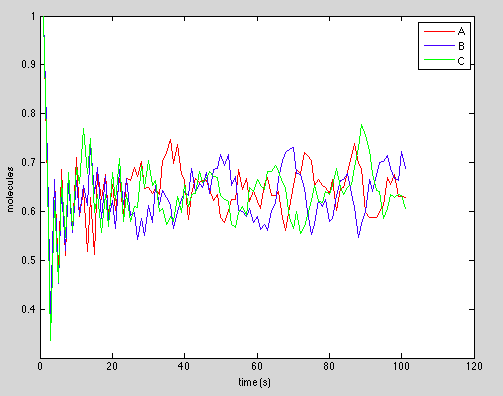
\includegraphics[scale=0.4]{repress_graph.png}
\caption{Average over many timecourses of the RNA-repressilator. The
rate of production and degradation at each time (seconds) step would
not be experimentally validateable (oscillations too small). }
\end{figure}
%----------------------------------------------------------------------------------------

\end{document}